% Created 2023-08-30 Wed 21:59
% Intended LaTeX compiler: lualatex
\documentclass[11pt]{article}
\usepackage{graphicx}
\usepackage{longtable}
\usepackage{wrapfig}
\usepackage{rotating}
\usepackage[normalem]{ulem}
\usepackage{amsmath}
\usepackage{amssymb}
\usepackage{capt-of}
\usepackage{hyperref}
\DeclareExerciseCollection{ListaMoleMassa}
\DeclareExerciseCollection{ListaBalan}
\DeclareExerciseCollection{ListaEstequiometria}
\DeclareExerciseCollection{ListaSolucoes}
\DeclareExerciseCollection{ListaTermoquimica}
\DeclareExerciseCollection{ListaLeiHess}
\DeclareExerciseCollection{ListaEquilibrio}
\DeclareExerciseCollection{ListaVolumetria}
\DeclareExerciseCollection{BalanceamentoRedox}
\author{fabio}
\date{\today}
\title{}
\hypersetup{
 pdfauthor={fabio},
 pdftitle={},
 pdfkeywords={},
 pdfsubject={},
 pdfcreator={Emacs 28.1 (Org mode 9.5.2)}, 
 pdflang={English}}
\begin{document}

\tableofcontents

\collectexercises{ListaBalan}
\begin{exercise}
Balanceie as reações químicas:
\begin{choice}(1)
\choice \ch{\lh Fe + \lh C$\ell$2 -> \lh FeC$\ell$3} \bigskip \bigskip
\choice \ch{\lh Fe + \lh O2 -> \lh Fe2O3} \bigskip \bigskip
\choice \ch{\lh FeBr3 + \lh H2SO4 -> \lh Fe2(SO4)3 + \lh HBr}\bigskip \bigskip
\choice \ch{\lh C4H6O3 + \lh H2O  ->  \lh C2H4O2} \bigskip \bigskip
\choice \ch{\lh C2H4 + \lh O2 -> \lh CO2 + \lh H2O} \bigskip \bigskip
%\choice \ch{\lh C4H10O + \lh O2 -> \lh CO2 + \lh H2O} \bigskip \bigskip
\choice \ch{\lh C7H16 + \lh O2 -> \lh  CO2 + \lh  H2O} \bigskip \bigskip
%\choice \ch{\lh H2SiC$\ell$2 + \lh H2O -> \lh H8Si4O4 + \lh HC$\ell$} \bigskip \bigskip
%\choice \ch{\lh HSiC$\ell$3 + \lh H2O -> \lh H10Si10O15 + \lh HC$\ell$} \bigskip \bigskip
\choice \ch{\lh C7H9 + \lh HNO3 -> \lh C7H6(NO2)3 + \lh H2O} \bigskip \bigskip
%\choice \ch{\lh C5H8O2 + \lh NaH + \lh HCl -> \lh C5H12O2 + \lh NaC$\ell$} \bigskip \bigskip
\choice \ch{\lh Fe + \lh H2SO4 \ -> \lh Fe2(SO4)3 + \lh H2} \bigskip \bigskip
\choice \ch{\lh C2H6 + \lh O2 -> \lh H2O + \lh CO2} \bigskip  \bigskip
\choice \ch{\lh KOH + \lh H3PO4 -> \lh K3PO4 + \lh H2O} \bigskip \bigskip
\choice \ch{\lh SnO2 + \lh H2 -> \lh Sn + \lh H2O} \bigskip \bigskip
\choice \ch{\lh NH3 + \lh O2 -> \lh NO  + \lh  H2O} \bigskip \bigskip
\choice \ch{\lh KNO3 + \lh H2CO3 -> \lh K2CO3 + \lh HNO3} \bigskip \bigskip 
\choice \ch{\lh B2Br6 + \lh HNO3 -> \lh  B(NO3)3 + \lh HBr} \bigskip \bigskip
\choice \ch{\lh BF3 + \lh  Li2SO3 -> \lh B2(SO3)3 + \lh LiF} \bigskip \bigskip
\choice \ch{\lh (NH4)3PO4 + \lh  Pb(NO3)4  -> \lh Pb3(PO4)4  + \lh NH4NO3} \bigskip \bigskip
%%\choice \ch{\lh SeC$\ell$6  + \lh  O2 -> \lh  SeO2 + \lh C$\ell$2} \bigskip \bigskip
\choice \ch{\lh HC$\ell$O4 + \lh P4O10  -> \lh H3PO4 + \lh C$\ell$2O7} \bigskip \bigskip
\choice \ch{\lh Ca3(PO4)2  + \lh H2SO4 -> \lh CaSO4  + \lh Ca(H2PO4)2} \bigskip \bigskip
%%\choice \ch{\lh FeO3  + \lh CO -> \lh Fe  + \lh CO2} \bigskip \bigskip
\choice \ch{\lh CO + \lh H2 -> \lh  C8H18 + \lh H2O}
\end{choice}
\end{exercise}

\collectexercisesstop{ListaBalan}


\collectexercises{ListaMoleMassa}
\begin{exercise}
Para o exercício, utilize esses valores como massa atômica relativa dos elementos químicos:

\textbf{H = 1; C = 12; N = 14; O = 16; Na = 23; Ca = 40; K = 39; C\(\ell\) = 35,5; P = 31;Cu = 63,5; S = 32; F = 19; Ag = 1O8; Al = 27; Fe = 56; I = 127.}


Determine as massas moleculares das substâncias abaixo:
\begin{choice}(3)
\choice \ch{N2}
\choice \ch{CO2}
\choice \ch{HNO3}
\vspace{3cm}
\choice \ch{H2SO4}
\choice  \ch{C6H12O6}
\choice \ch{Ca(OH)2}
\vspace{3cm}
\choice \ch{Ca(C$\ell$O3)2}
\choice \ch{(NH4)2SO4}
\choice \ch{Ca3(PO4)2}
\vspace{3.0cm}
\choice \ch{A$\ell$(OH)3}
\choice \ch{K4[Fe(CN)6]}
\vspace{3.5cm}
\end{choice}
\end{exercise}




\begin{exercise}
Determine a número de mols substâncias abaixo, utilize os dados da questão anterior:
\begin{choice}(2)
\choice 200 g de \ch{N2}
\choice 100 g de \ch{CO2}
\vspace{3.5cm}
\choice 25 g de \ch{HNO3}
\choice 687 g de \ch{H2SO4}
\vspace{3.5cm}
\choice  1,8 Kg de \ch{C6H12O6}
\choice 90g de \ch{Ca(OH)2}
\vspace{3.0cm}
\choice 500 g de \ch{Ca(C$\ell$O3)2}
\vspace{3.5cm}
\choice 5 g de \ch{(NH4)2SO4}
\choice 40 g de \ch{Ca3(PO4)2}
\vspace{3.5cm}
\choice 10 g de \ch{A$\ell$(OH)3}
\choice \ch{K4[Fe(CN)6]}
\end{choice}
\end{exercise}


\begin{exercise}
A magnetita, um minério do qual se extrai ferro possui fórmula molecular  \ch{Fe3O_x} e sua massa molecular é 232u. Determine o valor de \(x\) e escreva a fórmula molecular corretada magnetita.
\end{exercise}
\collectexercisesstop{ListaMoleMassa}




\collectexercises{ListaEstequiometria}


\begin{exercise}
Determine a massa de hidróxido de lítio produzida quando 0,38 gramas de lítio nitreto reage com a água de acordo com a seguinte equação química \textbf{desbalanceada}:

\begin{reaction*}
Li3N_{\sld} + H2O_{\lqdd} -> NH3_{\gas} + LiOH_{\aq}
\end{reaction*}

\blank[blank-style={\phantom{#1}},width=8\linewidth]{}
\end{exercise}
\begin{solution}
A
\end{solution}






\begin{exercise}
Num recipiente foram colocados 15g de ferro e 4,8g de oxigênio, conforme a reação \textbf{NÃO} balanceada. Qual a massa de \ch{Fe2O3} formada após um deles ser completamente consumido? (Fe = 56 g/mol; O\textsubscript{2} = 32 g/mol; \ch{Fe2O3}=160 g/mol).
\begin{reaction*}
Fe_{\sld} + O2_{\gas} -> Fe2O3_{\sld}
\end{reaction*}


\blank[blank-style={\phantom{#1}},width=8\linewidth]{}
\end{exercise}

\begin{solution}
Para a reação balanceada temos:

\begin{reaction*}
4 Fe_{\sld} + 3 O2_{\gas} -> 2 Fe2O3_{\sld}
\end{reaction*}

\begin{align*}
& 3 \cdot 32 ~~\text{\small \ch{O2}} -\!\!\!-\!\!\!- 2 \cdot 160~\text{\small \ch{Fe2O3}}\\
& 4,8~\text{\small \ch{O2}} -\!\!\!-\!\!\!- x~\text{\small \ch{Fe2O3}}\\
& x= 16 g
\end{align*}
\end{solution}

\begin{exercise}
O alumínio é obtido pela eletrólise da bauxita. Nessa eletrólise, ocorre a formação de oxigênio que reage com um dos eletrodos de
carbono utilizados no processo. A equação \textbf{não balanceada} que representa o processo global é:
\begin{reaction*}
A$\ell$2O3 + C -> CO2 + A$\ell$
\end{reaction*}
Para dois mols de \ch{A$\ell$2O3}, quantos mols de \ch{CO2} e de
 A$\ell$, respectivamente, são produzidos nesse
processo? Dados:  A$\ell$=27; C=12; O=16.


\blank[blank-style={\phantom{#1}},width=8\linewidth]{}
\end{exercise}

\begin{solution}
3 mol de CO\textsubscript{2} e 4 mol de A\(\ell\)
\end{solution}

\begin{exercise}
Em alguns fogos de artifício, alumínio metálico em pó é queimado, libertando luz e calor. Este fenômeno pode ser representado como:
\begin{reaction*}
4 Al_{\sld} + 3 O2_{\gas} -> 2 Al2O3_{\sld}
\end{reaction*}
Qual o volume de O\textsubscript{2}, nas CNTP, necessário para
reagir com 1 g do metal?
(Dado: Massa molar do  A\(\ell\) = 27 g/mol; Volume molar
nas CNTP = 22,4 L/mol).


\blank[blank-style={\phantom{#1}},width=8\linewidth]{}
\end{exercise}

\begin{solution}
0,62 L
\end{solution}


\begin{exercise}
A equação a seguir representa a obtenção de ferro pela reação de hematita com carvão:
\begin{reaction*}
Fe2O3 + 3 C -> 2 Fe + 3 CO
\end{reaction*}
(Dados: Massa molar do \ch{Fe2O3} = 160 g/mol; Massa
molar do Fe = 56 g/mol)
\begin{choice}
\choice Quantos quilogramas de hematita são necessários
para produzir 1120 kg de Fe? \bigskip


\blank[blank-style={\phantom{#1}},width=12\linewidth]{}


\choice Calcule, em condições ambientes, quantos litros
de CO são obtidos por mol de Fe produzido. (Dado:
volume molar nas condições ambientes = 24 L/mol).


\blank[blank-style={\phantom{#1}},width=8\linewidth]{}
\end{choice}
\end{exercise}

\begin{solution}

\end{solution}


\collectexercisesstop{ListaEstequiometria}




\collectexercises{ListaSolucoes}


\begin{exercise}
Calcule o massa em gramas necessários para preparar 250mL de solução \(1,5 \cdot 10^{-2}\) molar de
NaOH. Dados: NaOH= 40 g/mol
\end{exercise}




\begin{exercise}
Foi acrescentado 500 mL de água a uma solução aquosa de ácido sulfúrico de volume inicial igual a 200 mL e concentração de 20 g/L. Qual a concentração da solução após essa diluição?
\end{exercise}




\begin{exercise}
São dissolvidos 42,6 gramas de \ch{A$\ell$(NO3)3} em água de modo que o volume da solução seja igual a 4 litros. Qual a concentração molar dessa solução? Dado: \ch{A$\ell$(NO3)3} = 212 g/mol.
\end{exercise}



\begin{exercise}
Num balão volumétrico de 250mL adicionam-se 2,00g de sulfato de amônio sólido; o volume é completado com água. Calcule a concentração da solução obtida em g/L
\end{exercise}




\begin{exercise}
Descreva o procedimento para preparar uma solução de ácido acético, conhecido como vinagre, \ch{CH3COOH} com concentração de 0,05 para 250 mL de solução. MM = 60,1g, d = 1,05g/ml, Título = 99\%.
\end{exercise}


\collectexercisesstop{ListaSolucoes}







\collectexercises{ListaTermoquimica}

\begin{exercise}[points=1.0]
Quando o hidrogenocarbonato de sódio sólido é adicionado a uma solução de ácido cítrico em água, ocorre uma reação química. Essa reação altera a temperatura da água, que pode ser medida com um termômetro, conforme mostrado no diagrama

\begin{center}
\includegraphics[scale=.3]{../Listas/termometro.png}
\end{center}


Por que essa reação altera a temperatura da água?
\begin{choice}
\choice A reação é endotérmica porque as ligações nos produtos são mais fortes no total do que aquelas nos reagentes.
\choice A reação é exotérmica porque as ligações nos produtos são mais fortes no total do que aquelas nos reagentes.
\choice A reação é endotérmica porque as ligações nos produtos são mais fracas no total do que aquelas nos reagentes.
\choice A reação é exotérmica porque as ligações nos produtos são mais fracas no total do que aquelas nos reagentes.
\choice A moléculas rompem as ligações e a temperatura externa altera a reação química.
\end{choice}
\end{exercise}
\begin{solution}
D
\end{solution}


\begin{exercise}[points=1.0]
Qual dos seguintes valores é equivalente a  $\Delta$H$_3$. 
\begin{center}
\begin{tikzpicture}[
squarednode/.style={rectangle, draw=black!60, fill=red!5, very thick, minimum size=5mm}, shorten >=2pt,node distance=3cm,on grid,auto
]
\node[squarednode] (1) {A+B};
\node[squarednode] (2) [right=of 1] {C};
\node[squarednode] (3) [below=of 1] {F+G};
\node[squarednode] (4) [right= of 3] {E};
%%% 
%% Lines
\draw[->] (1.east) -- node[above]{$\Delta$H$_1$}(2.west);
\draw[->] (1.south) -- node[sloped, anchor=center, below]{$\Delta$H$_2$}(3.north);
\draw[->] (3.east) -- node[below]{$\Delta$H$_3$}(4.west);
\draw[->] (4.north) -- node[sloped, anchor=center, below]{$\Delta$H$_4$}(2.south);
\end{tikzpicture}
\end{center}

\begin{choice}(2)
\choice $\Delta$H$_1$ + $\Delta$H$_2$ + $\Delta$H$_4$
\choice $\Delta$H$_1$ - $\Delta$H$_2$ - $\Delta$H$_4$
\choice $\Delta$H$_1$ + $\Delta$H$_2$ - $\Delta$H$_4$
\choice $- \Delta$H$_1$ - $\Delta$H$_2$ - $\Delta$H$_4$
\choice $- \Delta$H$_1$ + $\Delta$H$_2$ + $\Delta$H$_4$
\end{choice}
\end{exercise}
\begin{solution}
B
\end{solution}



\begin{exercise}[points=1.0]
Qual das alternativas a seguir é a melhor descrição dessa reação química?
\begin{center}
\begin{endiagram}[
x-label=right,
y-label= above, y-label-text = Energia,
x-label= below, x-label-text = Progresso da Reação]
\ENcurve{4,4,4,-1,-1,-1}
\end{endiagram}
\end{center}
\begin{choice}
\choice A energia é liberada pela reação e os produtos são menos estáveis que os reagentes.
\choice A energia é absorvida pela reação e os produtos são menos estáveis que os reagentes.
\choice A energia é liberada pela reação e os produtos são mais estáveis que os reagentes.
\choice A energia é absorvida pela reação e os produtos são mais estáveis que os reagentes.
\choice A energia é constante 
\end{choice}
\end{exercise}
\begin{solution}
D
\end{solution}



\begin{exercise}[points=1.0]
Conhecendo a informações abaixo:
\begin{reactions}
Co_{\sld} + 1/2 O2_{\gas} -> CoO_{\sld} & $\qquad \enthalpy[unit=\kilo\joule]{-238}$\\
3 CoO_{\sld} + 1/2 O2_{\gas} -> Co3O4_{\sld} &  $\qquad \enthalpy[unit=\kilo\joule]{-177}$
\end{reactions}

Qual o valor da entalpia padrão da reação a seguir
\begin{reaction*}
Co3O4_{\sld} ->  3 Co_{\sld} + 2 O2_{\gas}
\end{reaction*}

Qual altertiva corresponde o valor correto de entalpia


\begin{choice}(2)
\choice \(\enthalpy[unit=\kilo\joule]{61}\)
\choice \(\enthalpy[unit=\kilo\joule]{-61}\)
\choice \(\enthalpy[unit=\kilo\joule]{891}\)
\choice \(\enthalpy[unit=\kilo\joule]{-891}\)
\choice \(\enthalpy[unit=\kilo\joule]{-560}\)
\end{choice}
\end{exercise}


\begin{exercise}[points=1.0]
O metano é um poluente atmosférico e sua combustão completa é descrita pela
equação química balanceada e pode ser esquematizada pelo diagrama abaixo.
\begin{reaction*}
CH4_{\gas} + 2 O2_{\gas} -> CO2_{\gas} + 2 H2O_{\gas}
\end{reaction*}
\begin{center}
\begin{endiagram}[
tikz         = {xscale=2.0}, scale        = 0.6,
y-label-offset=25pt,
y-label-text = Entalpia (kJ/mol),
x-label      = below,        x-label-text = progresso da reação,]
\ENcurve{5,8,0,0}
\AddAxisLabel{(N1-1)[965];(N1-2)[1215];(N1-3)[75]}
\ShowNiveaus[niveau=N1-1,shift=-0.5]
\ShowNiveaus[niveau=N1-3,shift=.5]
\draw[above left] (N1-1) ++ (0.6,1) node {\small \ch{CH4 + 2 O2} } ;
\draw[above] (N1-3) ++ (.8,0) node {\small\ch{CO2 + 2 H2O} } ;
\end{endiagram}
\end{center}
Sobre este processo químico, podemos afirmar que:
\begin{choice}
\choice a variação de entalpia é – 890 kJ/mol, e portanto é exotérmico.
\choice a entalpia de ativação é – 1140 kJ/mol.
\choice a variação de entalpia é – 1140 kJ/mol, e portanto é endotérmico.
\choice a entalpia de ativação é 890 kJ/mol.
\choice a entalpia de ativação é – 890 kJ/mol.
\end{choice}
\end{exercise}
\begin{solution}
A
\end{solution}

\begin{exercise}[points=1.0]
Observe o gráfico abaixo.
\begin{center}
\begin{endiagram}[
tikz         = {xscale=1.8}, scale        = 0.8,
y-label-offset=25pt,
y-label-text = Entalpia (kJ/mol),
x-label      = below,        x-label-text = progresso da reação,]
\ENcurve{1,1,11,5,5}
\AddAxisLabel{(N1-1)[0];(N1-4)[226];(N1-3)[560]}
\ShowNiveaus[niveau=N1-1,shift=-0.5]
\ShowNiveaus[niveau=N1-4,shift=.5]
\draw[above left] (N1-1) ++ (2,1) node {\small \ch{2 C_{(grafite)} + H2_{\gas}}} ;
\draw[above] (N1-4) ++ (.8,0) node {\small\ch{C2H2_{\gas}} } ;
\end{endiagram}
\end{center}
\begin{enumerate}
\item O gráfico corresponde a um processo endotérmico.
\item A entalpia da reação é igual a + 560 kcal.
\item A energia de ativação da reação é igual a 560 kcal.
\end{enumerate}

Está(ão) correta(s):
\begin{choice}(2)
\choice 1, apenas.
\choice 2, apenas.
\choice 2 e 3, apenas.
\choice 1 e 3, apenas.
\choice 1, 2 e 3.
\end{choice}
\end{exercise}
\begin{solution}
D
\end{solution}


\begin{exercise}[points=1.0]
O gráfico a seguir representa a variação de energia potencial quando o monóxido de
carbono, CO, é oxidado a CO\textsubscript{2} pela ação do NO\textsubscript{2}, de acordo com a equação:

\begin{reaction*}
CO_{\gas} + NO2_{\gas} -> CO2_{\gas} + NO_{\gas}
\end{reaction*}
\begin{center}
\begin{endiagram}[
tikz = {yscale=1.2}, scale = .9,
energy-step=50,
%energy-zero=0,
%energy-unit=\kilo\joule\per\mole,
AddAxisLabel/font = \footnotesize,
y-label-offset=25pt,
y-label-text = Entalpia (kJ/mol),
%y-label = above,
%y-label-text = $\Delta H$,
x-label= below, x-label-text = Progresso da Reação]
%\ENcurve{2,3,1}
\ENcurve{0,0,0,2.5,-4.5,-4.5,-4.5}
\AddAxisLabel*{-5;-4;-3;-2;-1;0;1;2;3;4}
\AddAxisLabel{(N1-2)[];(N1-4)[];(N1-6)[]}
\draw(1.7,.8)node{\ch{CO_{\gas} + NO2_{\gas}}};
\draw(10.5,-3.9)node{\ch{CO2_{\gas} + NO_{\gas}}};
\end{endiagram}

\end{center}
Com relação a esse gráfico e à reação acima, a afirmativa \textbf{CORRETA} é

\begin{choice}
\choice a energia de ativação para a reação direta é cerca de $\enthalpy{200}$.
\choice a reação inversa é exotérmica.
\choice em valor absoluto, o $\Delta$H da reação direta é cerca de $\enthalpy{360}$.
\choice em valor absoluto, o $\Delta$H da reação inversa é igual ao da reação direta.
\choice o $\Delta$H da reação direta é positivo.
\end{choice}
\end{exercise}
\begin{solution}
D
\end{solution}




\begin{exercise}[points=1.0]
O diagrama de entalpia para a combustão de 1,0 mol do gás propano ( \ch{C3H8}) pode ser representado através de 3 etapas.
\begin{center}

\begin{tikzpicture}[scale=1]
%\draw[step=1cm,black,very thin] (0,0) grid (10,10);
\draw[thick,-](0,0) -- (0,10); %% borda y
\draw[thick,-](11,10) -- (0,10); %% borda em top
\draw[thick,-](0,0) -- (11,0); %% borda  X
\draw[thick,-](11,0) -- (11,10); %% Eixo y2
%%%%  Line 
\draw[thick,-](2,8) -- (8,8);
\draw(5,8.5) node{\ch{3 C_{(grafite)} + 4 H2_{\gas} + 5 O2_{\gas}}};
\draw(5,7.8) node{\small \bfseries Elementos};
\draw[dashed,<-](2.9,8)--(2.9,6.0);
\draw(4.4,7.3) node[font={\footnotesize}]{\textcircled{1}Decomposição};
\draw(1.5,7) node[align=left, font={\small, \bfseries}]{$\Delta$H$_1$=\\ +103,85 kJ};
%%%% 
%%%% Line 2
\draw[thick,-](2,6) -- (6,6);
\draw(4.5,6.3) node{\ch{C3H8_{\gas} + 5 O2_{\gas}}};
\draw(4.4,5.8) node{\small \bfseries Reagentes};
\draw(8.4,7.3) node[font={\footnotesize}]{\textcircled{2} Formação de \ch{3 CO2_{\gas}}};
\draw(8.1,6.8) node[align=left, font={\small, \bfseries}]{$\Delta$H$_2$= -1181 kJ};
\draw[dashed,<-](2.9,8)--(2.9,6.0);
%%%% Line 3
\draw[thick,-](5,4) -- (9,4);
\draw(1.5,4) node[align=left, font={\small, \bfseries}]{$\Delta$H$^0_f$=\\ - 2220 kJ};
\draw[dashed,->](6.4,8)--(6.4,4.5);
\draw(7.5,4.3) node{\ch{3 CO2_{\gas} + 4 H2_{\gas} + 2 O2_{\gas}}};
%%%% Line 4
\draw[thick,-](2,2) -- (8,2);
\draw(5,1.7) node{\small \bfseries Produtos};
\draw(5,2.3) node{\ch{3 CO2_{\gas} + 4 H2O_{\lqdd}}};
\draw[thick,->](2.5,6)--(2.5,2.1);
\draw(9.3,3.3) node[font={\footnotesize}]{\textcircled{3} Formação de \ch{4 H2O}};
\draw[dashed,->](7.4,4)--(7.4,2.15);
\draw(9.1,2.7) node[align=left, font={\small, \bfseries}]{$\Delta$H$_3$= -1143 kJ};
%%%% Seta Eixo
\draw(-.3,5.5) node[sloped,anchor=center, rotate=90, above]{\large \bfseries Entalpia};
\draw[thick,->](-.6,6.5)--(-.6,7.5);

\end{tikzpicture}
\end{center}

Analisando o diagrama e utilizando seus conhecimentos de termoquímica pode-se afirmar que:

\begin{choice}
\choice a formação do propano gasoso libera cerca de 103,85 kJ/mol deste alcano.
\choice a formação de 72,0g de água gasosa apresenta um valor de ΔH de - 1.143 kj.
\choice a combustão completa de 26,0g de propano gasoso libera cerca de 2.220 kJ.
\choice a formação de 3 mols de dióxido de carbono gasoso libera cerca de 1.183 kcal.
\choice a formação de 4 mols de água libera cerca de 1.183 kcal.
\end{choice}
\end{exercise}
\begin{solution}
A
\end{solution}
\collectexercisesstop{ListaTermoquimica}





\collectexercises{ListaLeiHess}

\begin{exercise}
Calcule a entalpia de reação para a formação de cloreto de alumínio anidro, usando os dados abaixo:
% 2 CO2_{\gas} + H2O_{\lqdd}  & $\quad \enthalpy[unit=\kilo\joule]{-1300}$ \\
\begin{reactions*}
2 A$\ell$_{\sld}	+	6 HC$\ell$_{\aq} -> 2 A$\ell$C$\ell$3_{\aq}	+	3 H2_{\gas}	& $\quad \enthalpy[unit=\kilo\joule]{-1049}$\\	
HC$\ell$_{\gas} -> HC$\ell$_{\aq} & $\quad \enthalpy[unit=\kilo\joule]{-74}$\\
H2_{\gas}	+ C$\ell$2_{\gas}	->  2 HC$\ell$_{\gas} & $\quad \enthalpy[unit=\kilo\joule]{-185}$\\	
A$\ell$C$\ell$3_{\sld}	->  A$\ell$C$\ell$3_{\aq} & $\quad \enthalpy[unit=\kilo\joule]{-323}$
\end{reactions*}

Calcule o $\Delta$H da reação
\begin{reaction*}
2  A$\ell$_{\sld} + 3 C$\ell$2_{g} -> 2 A$\ell$C$\ell$3_{\sld} 
\end{reaction*}

\blank[blank-style={\phantom{#1}},width=12\linewidth]{}
\end{exercise}



\begin{exercise}
Use a Lei de Hess para calcular o $\Delta$H da reação
\begin{reaction*}
C4H8_{\gas} + 6 O2_{\gas} -> 4 CO2_{\gas} + 4 H2O_{\gas}
\end{reaction*}

A seguir as reações:


\begin{enumerate}[label=\Roman{*}.]
\item \ch{2 H2_{\gas} + O2_{\gas} -> 2 H2O_{\gas}}  $\qquad \enthalpy[unit=\kilo\joule]{-571}$
\item \ch{C4H8_{\gas} + H2_{\gas} -> C4H10_{\gas}} $\qquad \enthalpy[unit=\kilo\joule]{-126}$
\item \ch{2 C4H10_{\gas} + 13 O2_{\gas} -> 8 CO2_{\gas} + 10 H2O_{\gas}} $\qquad \enthalpy[unit=\kilo\joule]{-5754}$
\end{enumerate}


\blank[blank-style={\phantom{#1}},width=12\linewidth]{}
\end{exercise}
\begin{solution}
\end{solution}


\begin{exercise}
A seguir as entalpias de reações:

\begin{enumerate}[label=\Roman{*}.]
\item \ch{H2_{\gas} + F2_{\gas} -> 2 HF_{\gas}} $\qquad \enthalpy[unit=\kilo\joule]{-537}$
\item \ch{C_{\sld} + 2 F2_{\gas} -> CF4_{\gas}} $\qquad \enthalpy[unit=\kilo\joule]{-680}$
\item \ch{C_{\sld} + 2 H2_{\gas} -> C2H4_{\gas}} $\qquad \enthalpy[unit=\kilo\joule]{-52}$
\end{enumerate}


Calcule o $\Delta$H para a reação \textbf{NÃO BALANCEADA} abaixo.
\begin{reaction*}
C2H4_{\gas} +  F2_{\gas} -> CF4_{\gas} +  HF_{\gas}
\end{reaction*}

\blank[blank-style={\phantom{#1}},width=12\linewidth]{}
\end{exercise}
\begin{solution}
∆H = –1949
\end{solution}



\begin{exercise}
O diagrama a seguir 

\begin{center}
\tikzset{every picture/.style={line width=1.0pt}} %set default line width to 0.75pt        

\begin{tikzpicture}[x=0.75pt,y=0.75pt,yscale=-0.8,xscale=0.8]
%uncomment if require: \path (0,376); %set diagram left start at 0, and has height of 376

%Straight Lines [id:da4742405153664734] 
\draw    (108,307) -- (108,7) ;
\draw [shift={(108,5)}, rotate = 90] [color={rgb, 255:red, 0; green, 0; blue, 0 }  ][line width=0.75]    (10.93,-3.29) .. controls (6.95,-1.4) and (3.31,-0.3) .. (0,0) .. controls (3.31,0.3) and (6.95,1.4) .. (10.93,3.29)   ;
%Straight Lines [id:da4987255852646296] 
\draw    (108,307) -- (575,309.99) ;
\draw [shift={(577,310)}, rotate = 180.37] [color={rgb, 255:red, 0; green, 0; blue, 0 }  ][line width=0.75]    (10.93,-3.29) .. controls (6.95,-1.4) and (3.31,-0.3) .. (0,0) .. controls (3.31,0.3) and (6.95,1.4) .. (10.93,3.29)   ;
%Straight Lines [id:da8739968665747467] 
\draw    (138,76) -- (313,76) ;
%Straight Lines [id:da5716536683186184] 
\draw    (302,179) -- (479,181) ;
%Straight Lines [id:da12291859962824414] 
\draw    (142,270) -- (496,272) ;
%Straight Lines [id:da7467539186542762] 
\draw    (310,82) -- (308.04,170) ;
\draw [shift={(308,172)}, rotate = 271.27] [color={rgb, 255:red, 0; green, 0; blue, 0 }  ][line width=0.75]    (10.93,-3.29) .. controls (6.95,-1.4) and (3.31,-0.3) .. (0,0) .. controls (3.31,0.3) and (6.95,1.4) .. (10.93,3.29)   ;
%Straight Lines [id:da7999265194147146] 
\draw    (200,85) -- (200,260) ;
\draw [shift={(200,262)}, rotate = 270] [color={rgb, 255:red, 0; green, 0; blue, 0 }  ][line width=0.75]    (10.93,-3.29) .. controls (6.95,-1.4) and (3.31,-0.3) .. (0,0) .. controls (3.31,0.3) and (6.95,1.4) .. (10.93,3.29)   ;
%Straight Lines [id:da3547253027331094] 
\draw    (371,185) -- (370.03,260) ;
\draw [shift={(370,262)}, rotate = 270.74] [color={rgb, 255:red, 0; green, 0; blue, 0 }  ][line width=0.75]    (10.93,-3.29) .. controls (6.95,-1.4) and (3.31,-0.3) .. (0,0) .. controls (3.31,0.3) and (6.95,1.4) .. (10.93,3.29)   ;

% Text Node
\draw (75.6,108.52) node [anchor=north west][inner sep=0.75pt]  [rotate=-269.87,xscale=0.55,yscale=0.55] [align=left] {\Large Entalpia (KJ)};
% Text Node
\draw (145,44) node [anchor=north west][inner sep=0.75pt]  [xscale=0.55,yscale=0.55] [align=left] {\Large \ch{CH4_{\gas} + 2 O2_{\gas}}};
% Text Node
\draw (365,139) node [anchor=north west][inner sep=0.75pt]  [xscale=0.55,yscale=0.55] [align=left] {\Large \ch{CO_{\gas} + 2 H2O_{\lqdd} + 1/2 O2_{\gas}}};
% Text Node
\draw (414,245) node [anchor=north west][inner sep=0.75pt]  [xscale=0.55,yscale=0.55] [align=left] {\Large\ch{CO2_{\gas} + 2 H2O_{\lqdd}}};
% Text Node
\draw (215,108) node [anchor=north west][inner sep=0.75pt]  [xscale=0.55,yscale=0.55] [align=left] {\Large $\enthalpy[unit=\kilo\joule]{-607}$};
% Text Node
\draw (271,219) node [anchor=north west][inner sep=0.75pt]  [xscale=0.55,yscale=0.55] [align=left] {\Large $\enthalpy[unit=\kilo\joule]{-283}$};
% Text Node
\draw (145,162) node [anchor=north west][inner sep=0.75pt]  [xscale=0.55,yscale=0.55] [align=left] {\Large $\Delta$H$_r$ = ?};
% Text Node
\draw (393,318) node [anchor=north west][inner sep=0.75pt]  [xscale=0.55,yscale=0.55] [align=left] {\Large coordenada de reação};


\end{tikzpicture}
\end{center}

Analisando o diagrama qual o valor do $\Delta$H$_r$ para a reação \ch{CO2_{\gas} + 2 H2O_{\lqdd} -> CH4_{\gas} + 2 O2_{\gas}}.

\blank[blank-style={\phantom{#1}},width=12\linewidth]{}
\end{exercise}
\begin{solution}
\DeltaH=890 kJ
\end{solution}


\begin{exercise}
A oxidação do etanol leva à formação de ácido acético, levando ao vinagre é:

\begin{reaction*}
CH3CH2OH_{\lqdd} + O2_{\gas} -> CH3COOH_{\lqdd} + H2O_{\lqdd}
\end{reaction*}

Use os seguintes dados para calcular \$\(\Delta\)\$H\(_r^0\) (em kJ mol -1 )
\begin{reactions}
4C_{\sld} + 6 H2_{\gas} + O2_{\gas} -> 2 CH3CH2OH_{\lqdd}  &  $\qquad \enthalpy{-555}$  \\
2 C_{\sld} + 2 H2_{\gas} + O2_{\gas} -> CH3COOH_{\lqdd} &  $\qquad \entalphy{-484}$ \\
2 H2_{\gas} + O2_{\gas} -> 2 H2O_{\gas} &  $\qquad \enthalpy{-483}$ \\
H2O_{\lqdd} ->  H2O_{\gas} &  $\qquad \enthalpy{44}$
\end{reactions}
\end{exercise}




\collectexercises{ListaEquilibrio}


\begin{exercise}
Uma mistura de \ch{CO} e \ch{C$\ell$2} é colocada em um frasco de reação: [CO]=0,0102 mol/L e [\ch{C$\ell$2}]= 0,00609 mol/L Quando a reação: 

\begin{reaction*}
	CO_{\gas} +  C$\ell$2_{\gas} <=> COC$\ell$2_{\gas}
\end{reaction*}

atinge o equilíbrio a 600 K, a [\ch{C$\ell$2}]=0,00301 mol/L.


\begin{choice}
\choice Calcule as concentrações de CO e \ch{COC$\ell$2} no equilíbrio.

\blank[blank-style={\phantom{#1}},width=12\linewidth]{}

\choice Calcule o valor de \(k_c\)

\blank[blank-style={\phantom{#1}},width=7\linewidth]{}
\end{choice}
\end{exercise}


\begin{exercise}
A dissociação do iodo molecular em átomos de iodo é representada por


\begin{reaction*}
I2_{\gas} <=> 2 I_{\gas}
\end{reaction*}

A 1000 K, a constante de equilíbrio \(k_c\) da reação é \(3,80 \times 10^{-5}\). Admita que inicialmente as concentrações de 0,0456 mol de \ch{I2} em um frasco de 2,3 L. Quais as concentrações em equilíbrio?



\blank[blank-style={\phantom{#1}},width=7\linewidth]{}
\end{exercise}


\begin{solution}

\begin{tabular}{cc@{}c@{}c@{}c@{}c}
	\toprule
	&  \ce{Br2_{(g)}} \qquad  & ${}\leftrightharpoons{}$ \qquad & 2\ce{Br_{(g)}}  \\
	\midrule
	Início   &       0,0456 mol/2,3 L (0,0198 M)    &&   $\cdots$                           \\
	$\Delta$   &       $-x$                       &&  $ + 2x$    \\
	$[$Eq. final$]$   &    $0,0198 - x $         && $2x$  \\
	\bottomrule
\end{tabular}

$k_c=\displaystyle \frac{[\ce{I}]^2}{[\ce{I2}]} \Rightarrow$
$3,8 \times 10^{-5}=\displaystyle \frac{(2x)^2}{(0,01982-x)} \Rightarrow $
$ 4x^2 + 3,8 \times 10^{-5}x - 3,8 \times 10^{-7} = 0$ \\
$x'= 4,29 \times 10^{-4} $ \\ 
$x''= -4,0 \times 10^{-4}$ \\
$[\ce{I2}]_{eq.}=0,0198-4,29 \times 10^{-4}$ $\Rightarrow$ \\
\boxed{$$\rm [\ce{I2}]_{eq.}=0,01937$$\quad M} \\
$[\ce{I}]_{eq.}$= $2x'\Rightarrow 2 \times (4,29 \times 10^{-4}) \Rightarrow$\\
\boxed{$$\rm [\ce{I}]_{eq.} = 8,58 \times 10^{-4}$$\quad M} \\
\end{solution}


\begin{exercise}
O brometo de carbonila decompõe-se em monóxido de carbono e bromo:

\begin{reaction*}
COBr2_{\gas} <=> CO_{\gas} + Br2_{\gas}
\end{reaction*}

o valor de \(k_c\) é 0,190  a 73\textsuperscript{0}C. Se coloca 0,500 mol de \ch{COBr2} em um frasco de 2,00 L e se aquece. Quais serão as concentrações no equilíbrio de \ch{COBr2}, CO e \ch{Br2}? 

\vspace{5cm}
\end{exercise}



\begin{exercise}
Para a reação:
\begin{reaction*}
N2_{\gas} + 3 H2_{\gas} <=> 2 NH3_{\gas}
\end{reaction*}

foram adicionados inicialmente  1 mol de \ch{N2} e 1 mol de \ch{H2}. Após estabelecer o equilíbrio foram remanecente 0,60 mol de \ch{N2}. Calcule a constante de equilíbrio $k_c$ para a reação.
\end{exercise}



\collectexercisesstop{ListaEquilibrio}



\collectexercises{ListaVolumetria}



\begin{exercise}
Calcule o massa em gramas necessários para preparar 250mL de solução \(1,5 \cdot 10^{-2}\) molar de
NaOH. Dados: NaOH= 40 g/mol

\blank[blank-style={\phantom{#1}},width=8\linewidth]{}
\end{exercise}



\begin{exercise}
São dissolvidos 42,6 gramas de \ch{A$\ell$(NO3)3} em água de modo que o volume da solução seja igual a 4 litros. Qual a concentração molar dessa solução? Dado: \ch{A$\ell$(NO3)3} = 212 g/mol.

\blank[blank-style={\phantom{#1}},width=8\linewidth]{}
\end{exercise}



\begin{exercise}
Um produtor rural deseja aplicar um fertilizante em sua área agricola com fosfato diamonico \ch{(NH4)2HPO4}, 1 L com um concentração de 2 mol/L para m\textsuperscript{2} de área cultivada. Qual a massa em Kg de fosfato diamonico para fertilizar essa área? Dados: \ch{(NH4)2HPO4}=132,06 g/mol



\begin{center}
\tikzset{every picture/.style={line width=0.75pt}} %set default line width to 0.75pt        

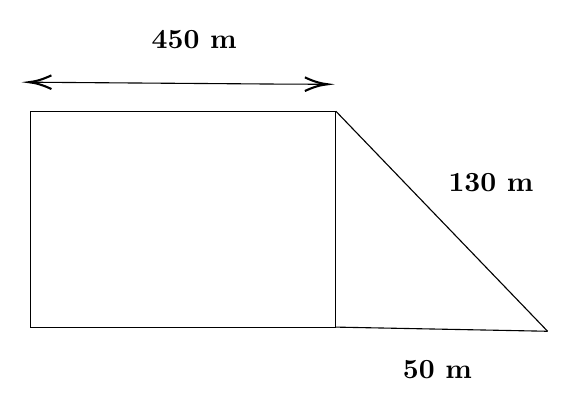
\begin{tikzpicture}[x=0.75pt,y=0.75pt,yscale=-1,xscale=1]
\draw   (162,124) -- (309,124) -- (309,228) -- (162,228) -- cycle ;
\draw    (309,124) -- (411,230) ;
\draw    (309,228) -- (411,230) ;
\draw    (161,110) -- (276.99,110.88) -- (282.01,110.92) -- (303,110.99) ;
\draw [shift={(305,111)}, rotate = 180.21] [color={rgb, 255:red, 0; green, 0; blue, 0 }  ][line width=0.75]    (10.93,-3.29) .. controls (6.95,-1.4) and (3.31,-0.3) .. (0,0) .. controls (3.31,0.3) and (6.95,1.4) .. (10.93,3.29)   ;
\draw [shift={(161,110)}, rotate = 0] [color={rgb, 255:red, 0; green, 0; blue, 0 }  ][line width=0.75]    (10.93,-3.29) .. controls (6.95,-1.4) and (3.31,-0.3) .. (0,0) .. controls (3.31,0.3) and (6.95,1.4) .. (10.93,3.29)   ;
% Text Node
\draw (219,84) node [anchor=north west][inner sep=0.75pt]   [align=left] {\textbf{450 m}};
% Text Node
\draw (340,243) node [anchor=north west][inner sep=0.75pt]   [align=left] {\textbf{50 m}};
% Text Node
\draw (362,153) node [anchor=north west][inner sep=0.75pt]   [align=left] {\textbf{130 m}};
\end{tikzpicture}
\end{center}
\end{exercise}


\collectexercisesstop{ListaVolumetria}




\collectexercises{BalanceamentoRedox}


\begin{exercise}
Realize o balanceamento das reações redox
\begin{choice}(1)
\choice \ch{As2O3 + NO3^- ->  H3AsO4 + N2O3} \vspace{1cm} 
\choice \ch{KI + KNO2 + H2SO4 ->  I2 + NO + K2SO4 + H2O}\vspace{1cm}
\choice \ch{KI + H2SO4 -> K2SO4 + I2 + H2S + H2O}  \vspace{1cm}
\choice \ch{C + H2SO4 -> CO2 + SO2 + H2O}  \vspace{1cm}
\choice \ch{Cu + SO4^{2-} -> Cu^{2+} + SO2}  \vspace{1cm}
\choice \ch{KSCN + H2O + I2 -> KHSO4 + HI + ICN}  \vspace{1cm}
\choice \ch{A$\ell$Br3 + KMnO4 + H2SO4 -> A$\ell$2(SO4)3 + K2SO4 + MnSO4 + Br2 + H2O}  \vspace{1cm}
\choice \ch{FeSO4 + KMnO4 + H2SO4 -> Fe2(SO4)3 + K2SO4 + MnSO4 + H2O}  \vspace{1cm}
\choice \ch{Na2C2O4 + KMnO4 + H2SO4 -> K2SO4 + Na2SO4 + MnSO4 + CO2 + H2O}
\end{choice}
\end{exercise}


\collectexercisesstop{BalanceamentoRedox}
\end{document}
